\documentclass[10pt]{beamer}
\usetheme[progressbar=frametitle]{metropolis}
\usepackage[utf8]{inputenc}
% \usepackage[utf8]{vietnam}

\usepackage{appendixnumberbeamer}

% \usepackage{pdfpages} % to include pdf
\usepackage{booktabs}
\usepackage[scale=2]{ccicons}
\usepackage{xcolor}
\usepackage{verbatim}
\usepackage{graphicx}
\usepackage{xspace}

\newcommand{\themename}{\textbf{\textsc{metropolis}}\xspace}

\usepackage{listings}


\title[Wild Pig Maze title]{Wild Pig Maze by Nob Yoshigahara}
\subtitle{An algorithmic approach}
% \date{\today}
\date{December 8, 2020}

\author[shortname]{
  Do Xuan Anh \\ % \inst{1} \\
  Le Quang Dung \\ % \inst{1} \\
  Hoang Anh Quan \\ % \inst{1} \\
  Trinh Huy Vu \\ % \inst{1} \\
  }
% \institute[shortinst]{\inst{1} VNU University of Science}
% \titlegraphic{\hfill\includegraphics[height=1.5cm]{logo.pdf}}


\begin{document}

\begin{frame}
	\maketitle
\end{frame}

\begin{frame}{Table of content}
	\setbeamertemplate{section in toc}[sections numbered]
	\tableofcontents[hideallsubsections]
\end{frame}

\section{Problem statements}

\begin{frame}{Problem statements}
  \begin{figure}[htb!] % HERE, here, top, bottom, page
    \centering
    % left, bottom, right, top
    % width=5\textwidth,height=5\textheight, keepaspectratio, angle=30, scale=1
    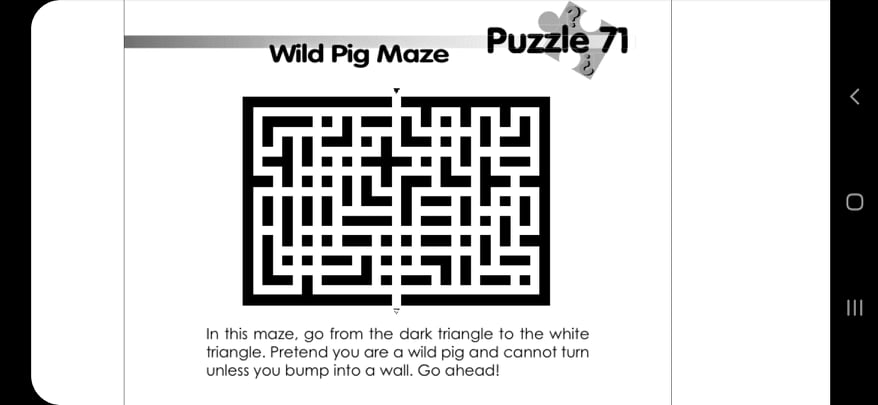
\includegraphics[trim={3cm 0cm 3cm 0cm},clip,scale=0.4]{../images/input_image.jpg}
    \caption{Nob Yoshigahara, Puzzles 101: A PuzzleMasters Challenge}
    % \caption[short caption]{long caption}
    \label{fig:} % label is given after caption
  \end{figure}
\end{frame}

\section{Algorithm}

\begin{frame}{Overview}
  \begin{enumerate}
    \item Creating a $(0, 1)$ - matrix from the image of the maze.
    \item Changing matrix to a directed graph.
    \item Find a path of the directed graph and draw it to the image.
  \end{enumerate}
\end{frame}

%----------------------STEP 1-------------------%
\begin{frame}{Step 1: Creating a $(0, 1)$ - matrix from the image of the maze}
Consist of THREE main stages:
\begin{itemize}
    \item [1)] Using PIL package to save the pixels of the image as a $(0, 1)$~-~matrix.
    \begin{figure}[htb!]
        \centering
        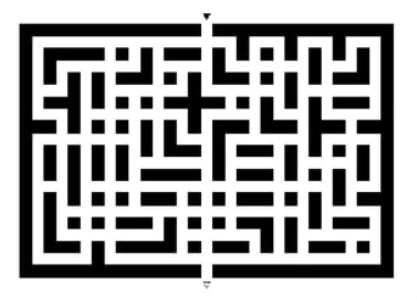
\includegraphics[scale=0.6]{../images/input_image2.jpg}
        \caption[]{The bordered maze.}
        \label{fig:} % label is given after caption
    \end{figure}
    \item [2)] Determining coordinates of four corners of the maze.
\end{itemize}
\end{frame}

\begin{frame}{Step 1: Creating a $(0, 1)$ - matrix from the image of the maze}
\begin{itemize}
    \item [3)] Shrinking the above $(0,1)$ - matrix into a smaller one (the desired~matrix).\\
    We have two approaches:
    \begin{itemize}
        \item Measure the width of the path.
        \begin{figure}[htb!]
            \centering
            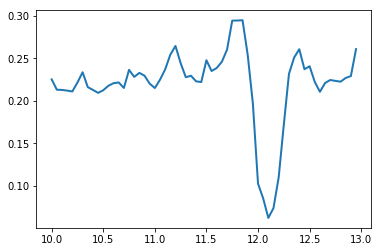
\includegraphics[scale=0.6]{../images/error1.png}
            \caption[]{Error corresponding to the path's width.}
            \label{fig:} % label is given after caption
        \end{figure}
    \end{itemize}
\end{itemize}
\end{frame}

\begin{frame}{Step 1: Creating a $(0, 1)$ - matrix from the image of the maze}
    \begin{itemize}
        \item Determine the suitable size of the matrix.
        \begin{figure}[htb!]
            \centering
            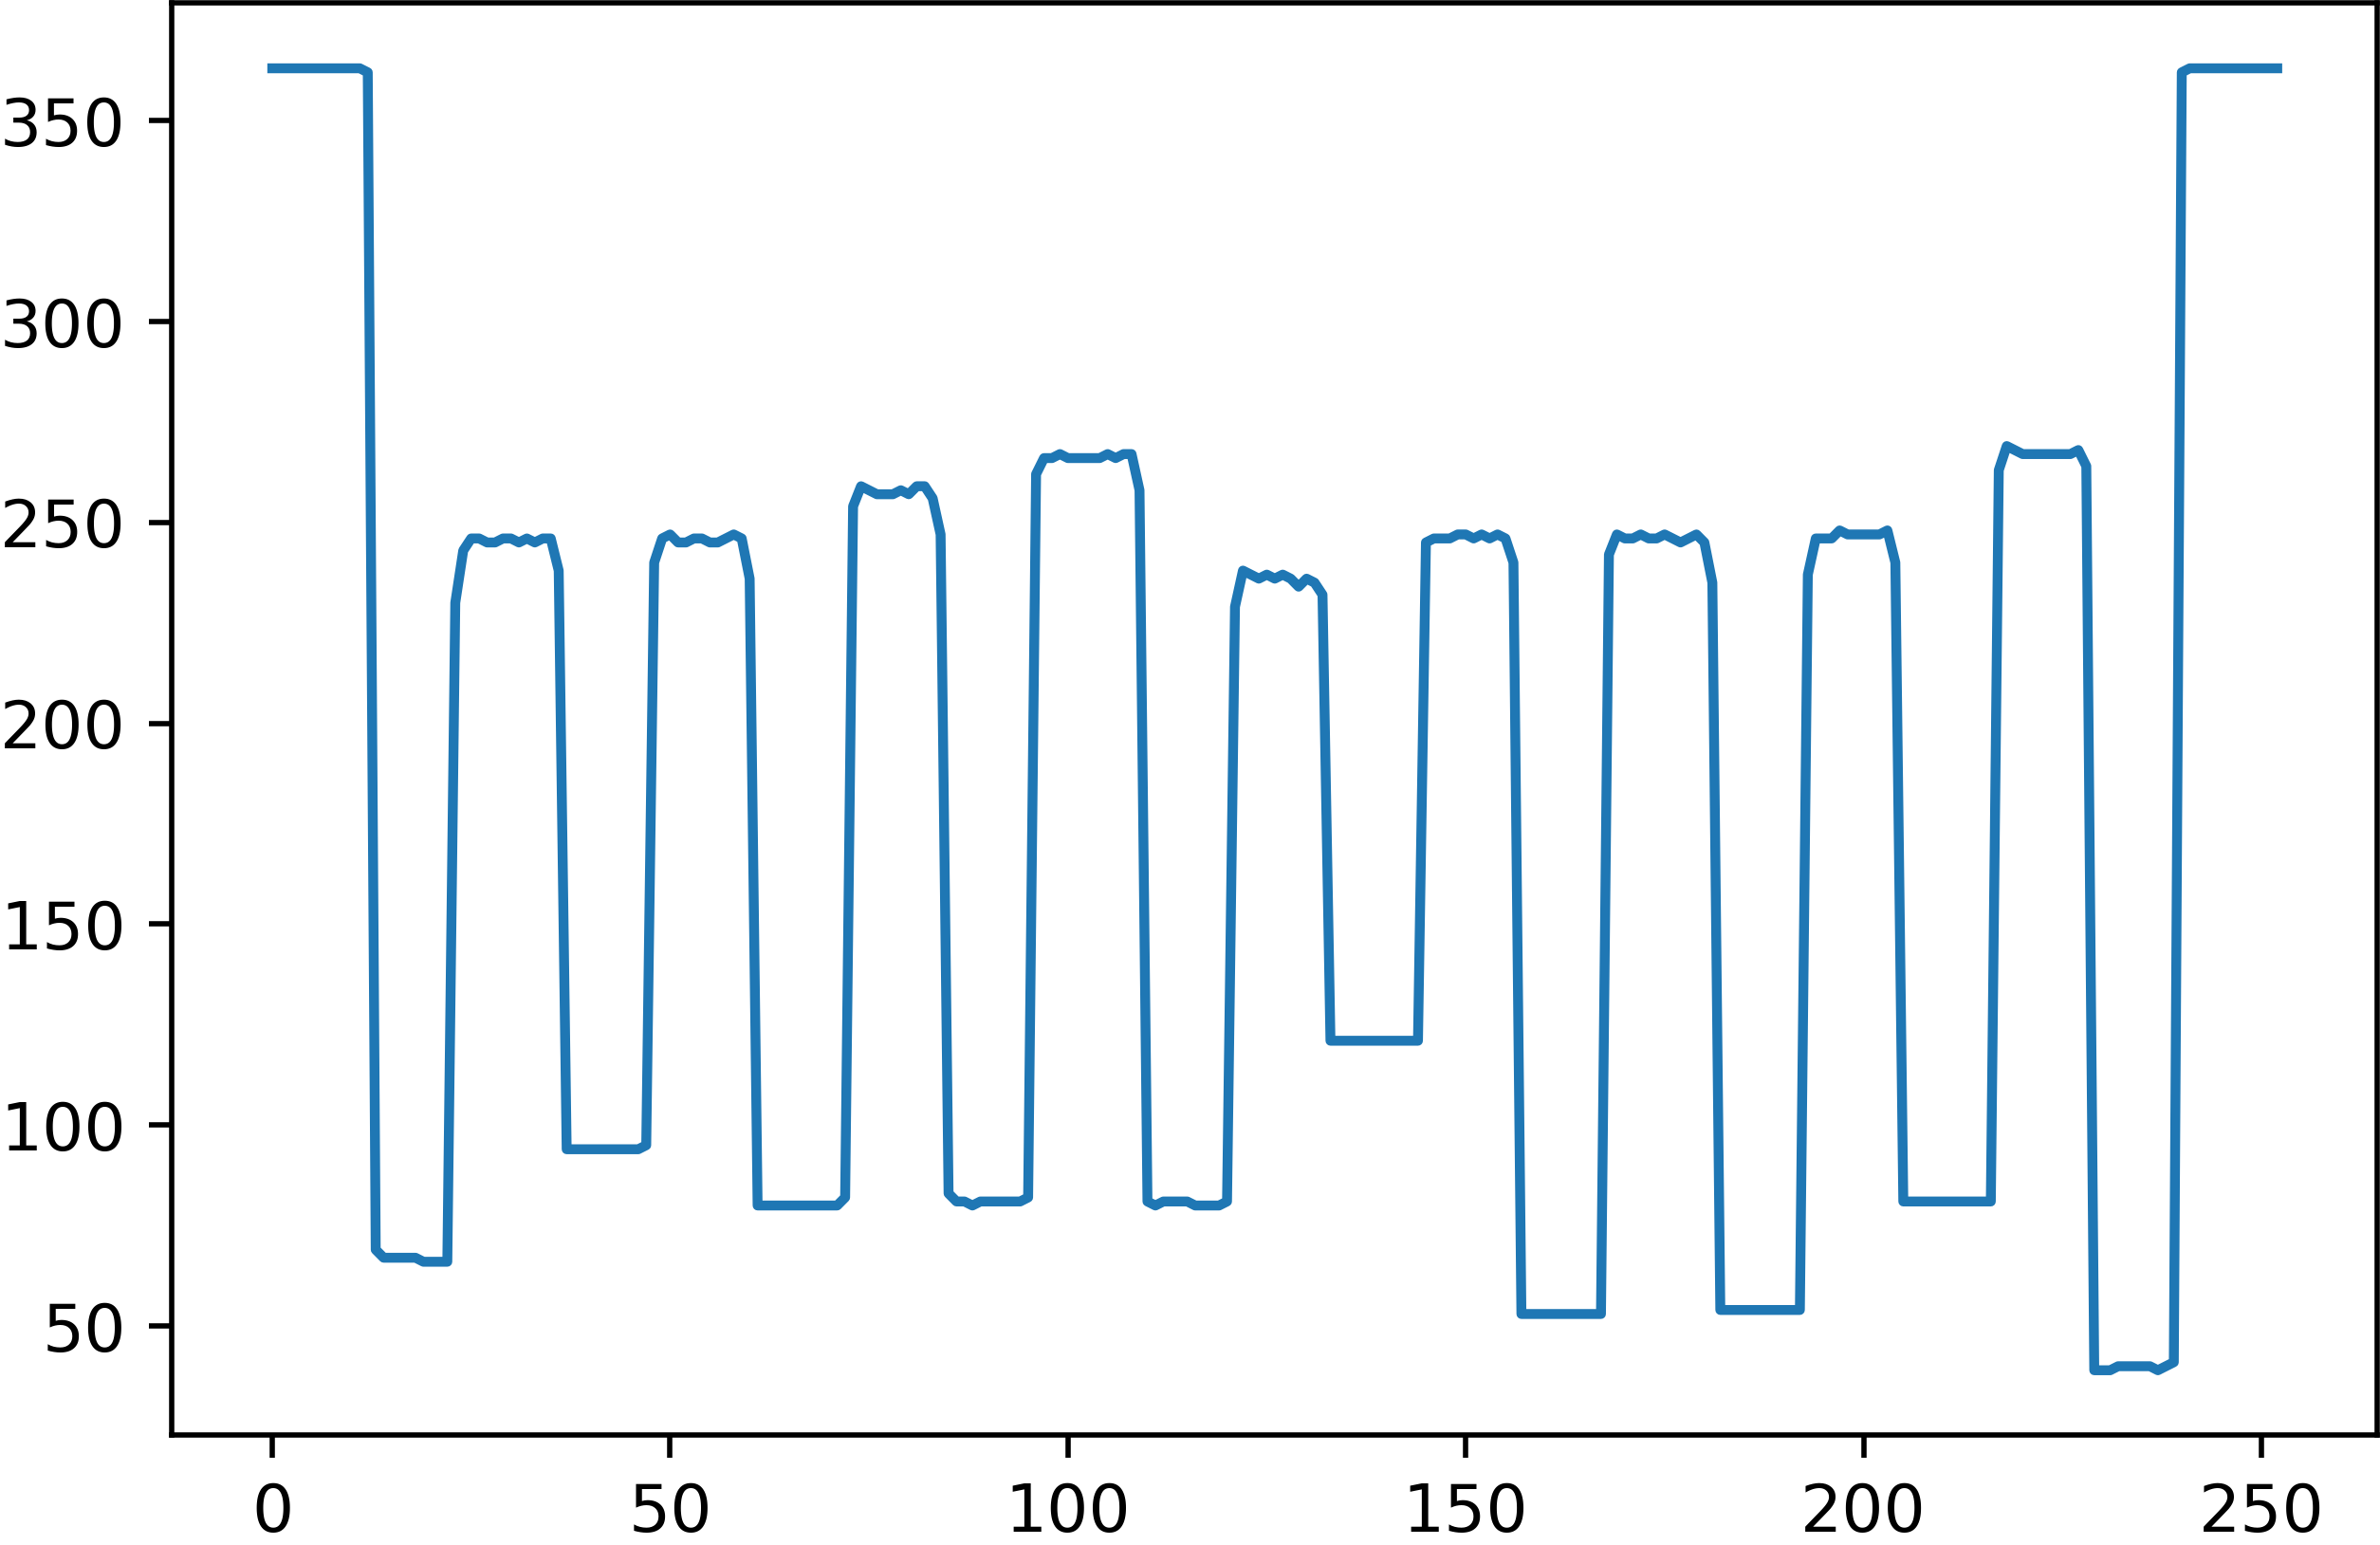
\includegraphics[scale=0.43]{../images/horizontal_sum.png}
            %\caption[]{Error corresponding to the path's width.}
            \label{fig:} % label is given after caption
        \end{figure}
        \begin{figure}[htb!]
            \centering
            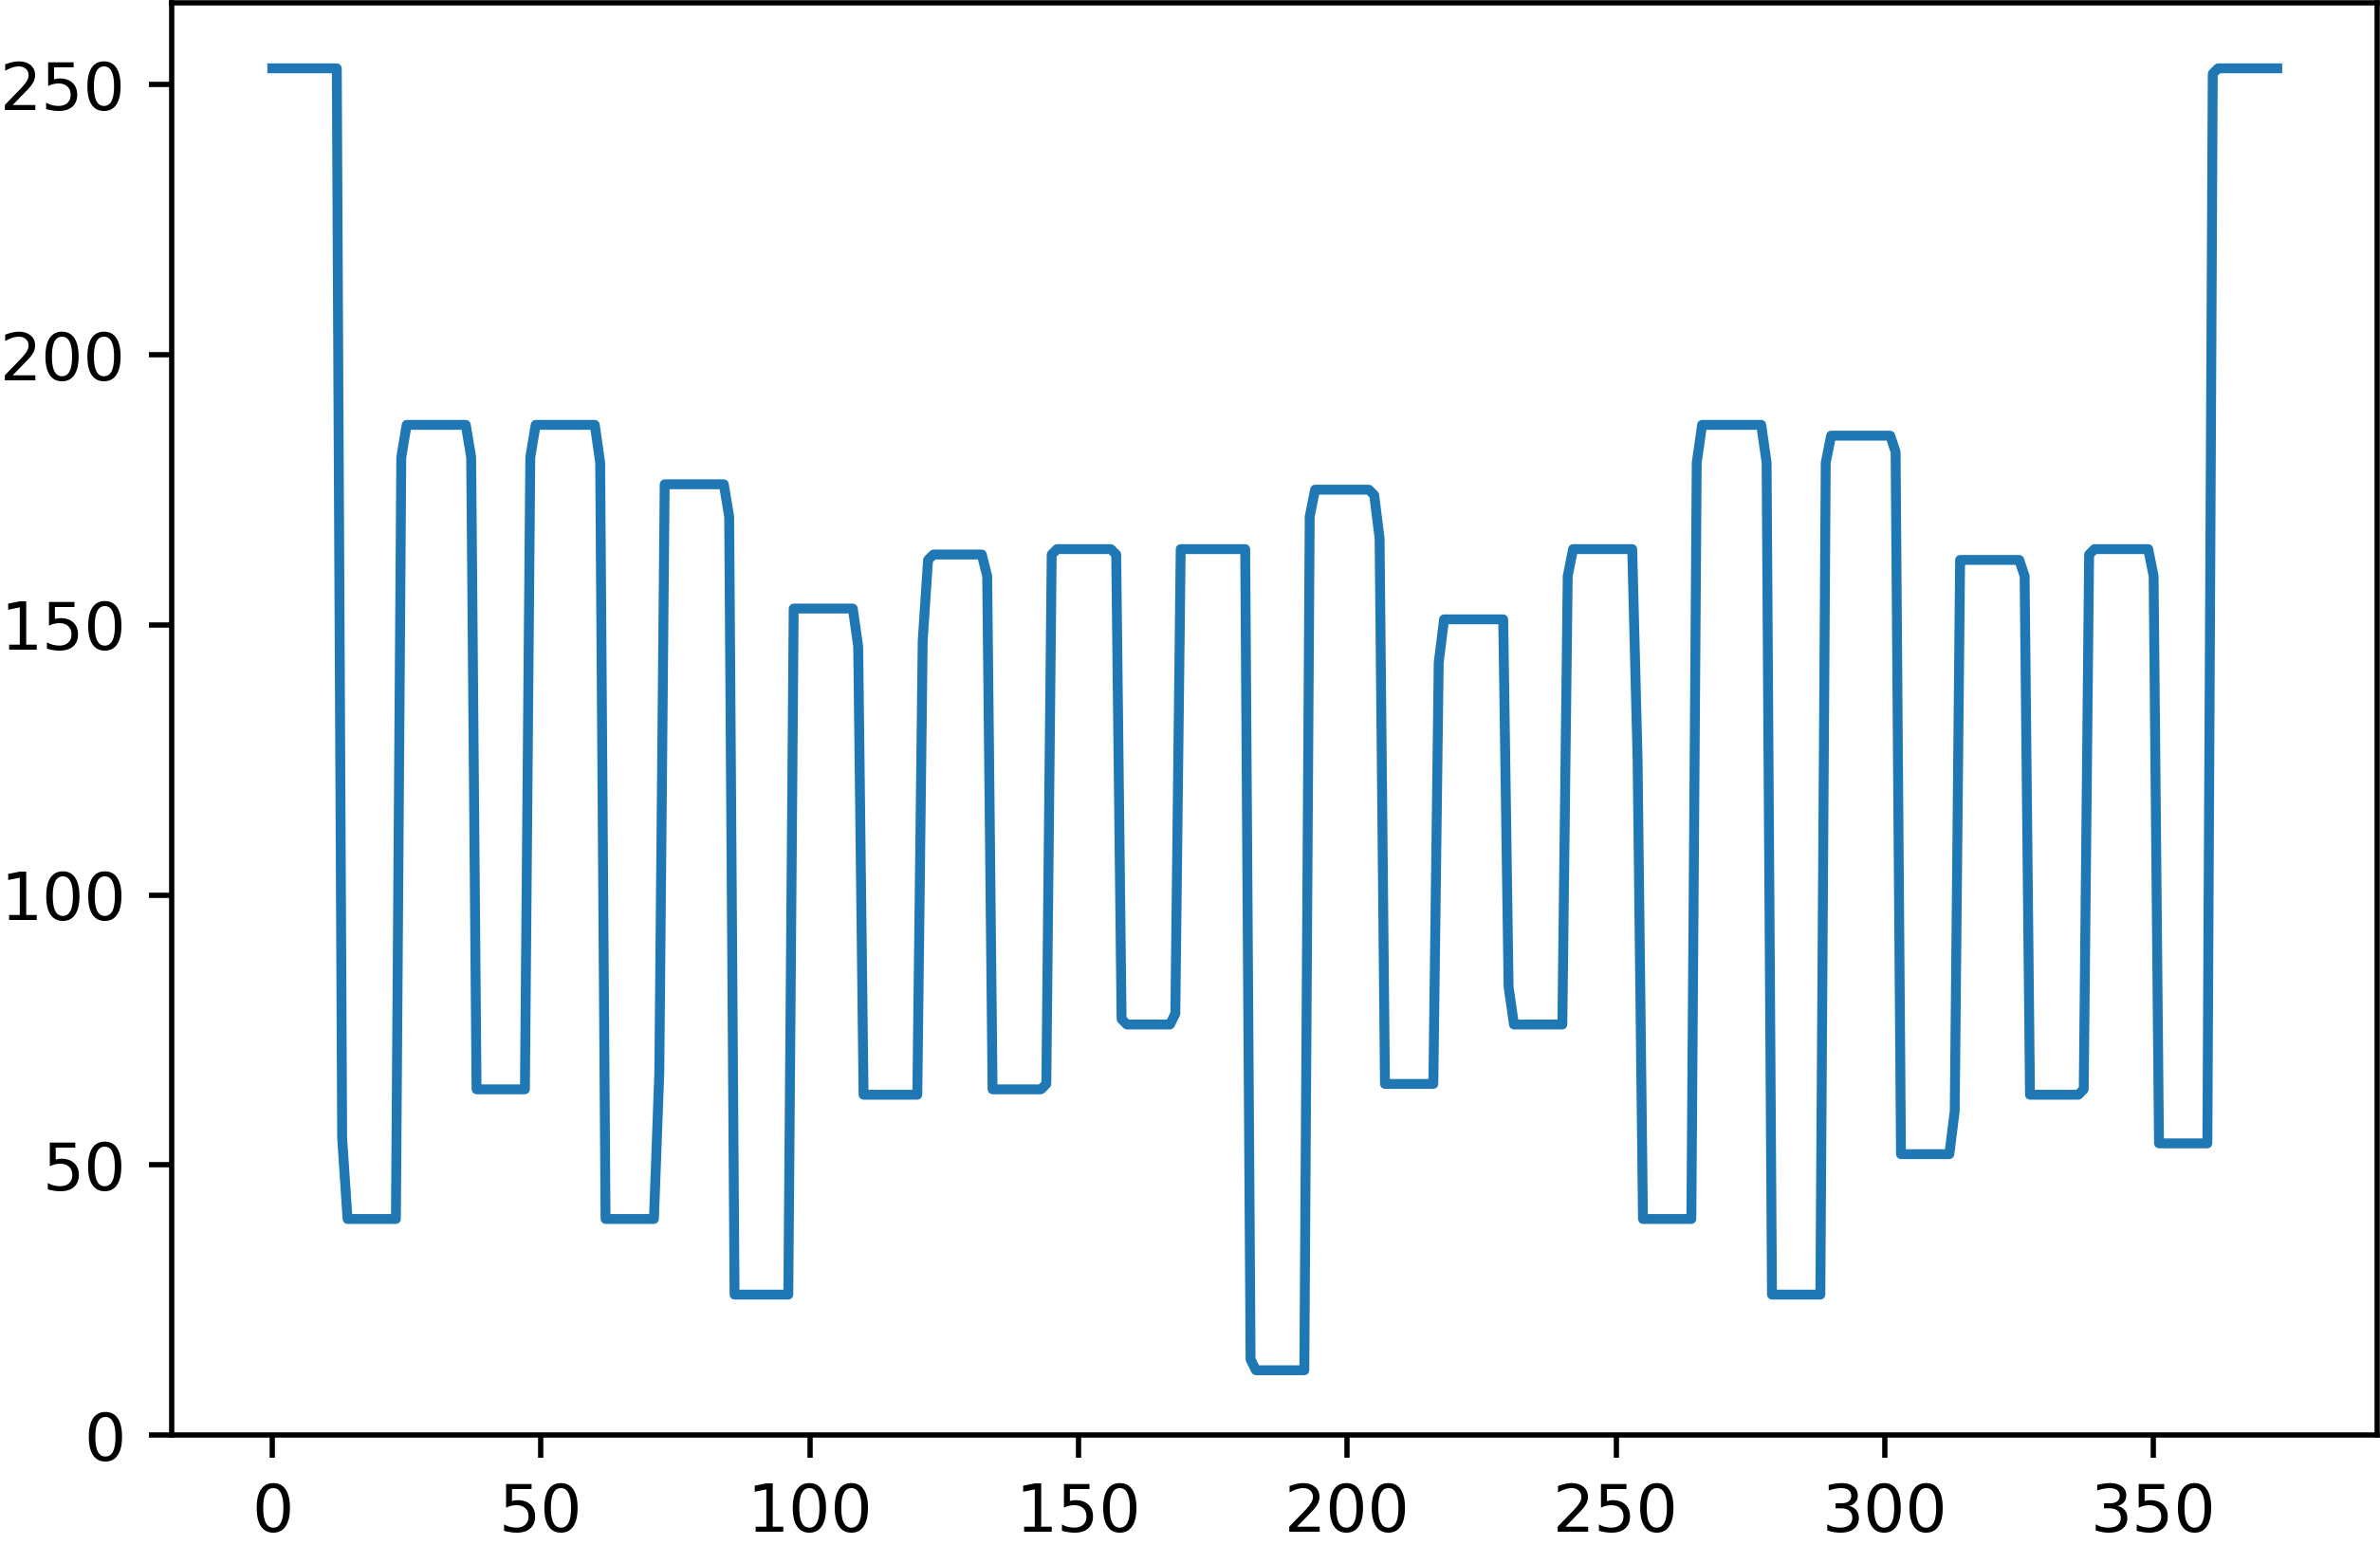
\includegraphics[scale=0.43]{../images/vertical_sum.png}
            \caption[]{The horizontal sum and vertical sum.}
            \label{fig:} % label is given after caption
        \end{figure}
    \end{itemize}
\end{frame}

%----------------------STEP 2-------------------%
\begin{frame}{Step 2: Changing matrix to a directed graph}
\begin{itemize}
    \item Create a graph G.
    \item For each position which is empty, we add four vertices to the graph, which imply the position from the previous step.
    \item Add nodes to the graph which follow some rules.
\end{itemize}
\end{frame}


%----------------------STEP 3-------------------%
\begin{frame}{Step 3: Find a path of the directed graph and visualize it}
\begin{itemize}
    \item Find a path of the directed graph which is output of Step 2.
    % \item Draw the path to the image by using the matplotlib package in Python.
    \item Visualize the path by using the matplotlib package in Python.
\end{itemize}
\end{frame}

\section{Results}

\begin{frame}{Path in the maze}
  \begin{figure}[htb!] % HERE, here, top, bottom, page
    \centering
    % left, bottom, right, top
    % width=5\textwidth,height=5\textheight, keepaspectratio, angle=30, scale=1
    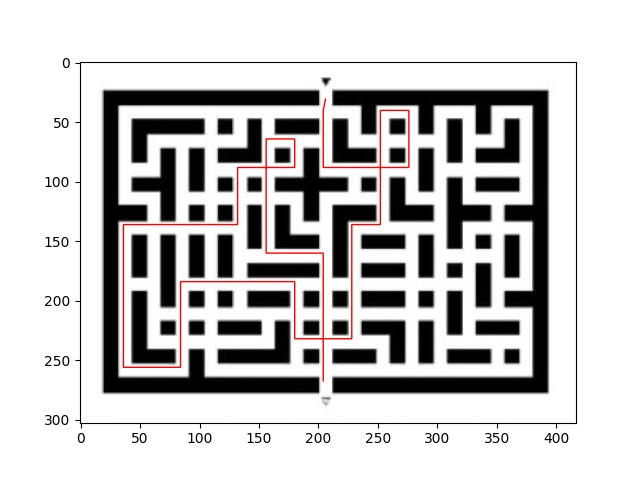
\includegraphics[trim={0cm 0cm 0cm 0cm},clip,scale=0.6]{../images/output_image.jpg}
    % \caption{Pat}
    % \caption[short caption]{long caption}
    \label{fig:} % label is given after caption
  \end{figure}

\end{frame}

\begin{frame}{Statistics}
  \begin{itemize}
    \item 379 lines of code.
    \item Commits counter:
    \begin{itemize}
      \item Do Xuan Anh: 11
      \item Le Quang Dung: 27
      \item Hoang Anh Quan: 11
      \item Trinh Huy Vu: 11
    \end{itemize}
  \end{itemize}
\end{frame}

\begin{frame}{What we have learned}
  \begin{itemize}
    \item Version control system: Git/Github.
    \item Packages in Python: matplotlib, networkx, numpy, PIL.
    \item Teamwork management.
  \end{itemize}
\end{frame}

% Local background must be enclosed by curly braces for grouping.
{\usebackgroundtemplate{
\includegraphics[width=\paperwidth]{../images/thank_you.jpg}}%
\begin{frame}{}
\end{frame}
}

\end{document}
